\documentclass[tikz,border=8pt]{standalone}
\usepackage{braket}

\begin{document}
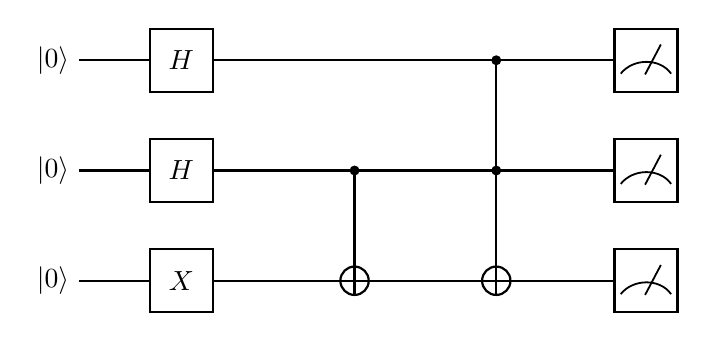
\begin{tikzpicture}[
  wire/.style={line width=0.8pt},
  gate/.style={draw,fill=white,line width=0.8pt,
    minimum width=0.8cm,minimum height=0.8cm,inner sep=0pt}
]
  \foreach \y in {1.4,0,-1.4} {
    \draw[wire] (0,\y) -- (7.2,\y);
    \node[left] at (0,\y) {$\ket{0}$};
    \node[gate] at (7.2,\y) {};
    % Measurement symbol: meter arc and pointer inside the gate box.
    \draw[line width=0.65pt] (6.88,\y-0.17)
      .. controls (7.04,\y+0.03) and (7.38,\y+0.03) .. (7.52,\y-0.17);
    \draw[line width=0.65pt] (7.19,\y-0.18) -- (7.39,\y+0.20);
  }

  \node[gate] at (1.3,1.4) {$H$};
  \node[gate] at (1.3,0) {$H$};
  \node[gate] at (1.3,-1.4) {$X$};

  % CNOT: the middle qubit controls the bottom qubit.
  \draw[wire] (3.5,-1.4) -- (3.5,0);
  \fill (3.5,0) circle (1.8pt);
  \draw[wire,fill=white] (3.5,-1.4) circle (0.18);
  \draw[wire] (3.32,-1.4) -- (3.68,-1.4);
  \draw[wire] (3.5,-1.58) -- (3.5,-1.22);

  % Toffoli: the top and middle qubits control the bottom qubit.
  \draw[wire] (5.3,-1.4) -- (5.3,1.4);
  \fill (5.3,1.4) circle (1.8pt);
  \fill (5.3,0) circle (1.8pt);
  \draw[wire,fill=white] (5.3,-1.4) circle (0.18);
  \draw[wire] (5.12,-1.4) -- (5.48,-1.4);
  \draw[wire] (5.3,-1.58) -- (5.3,-1.22);
\end{tikzpicture}
\end{document}
